\documentclass[12pt]{article}
\usepackage[top=1in,left=1in, right = 1in, footskip=1in]{geometry}

\usepackage{graphicx}
%\usepackage{adjustbox}

%% \newcommand{\comment}{\showcomment}
\newcommand{\comment}{\nocomment}

\newcommand{\showcomment}[3]{\textcolor{#1}{\textbf{[#2: }\textsl{#3}\textbf{]}}}
\newcommand{\nocomment}[3]{}

\newcommand{\jd}[1]{\comment{cyan}{JD}{#1}}
\newcommand{\swp}[1]{\comment{magenta}{SWP}{#1}}

\newcommand{\eref}[1]{Eq.~\ref{eq:#1}}
\newcommand{\fref}[1]{Fig.~\ref{fig:#1}}
\newcommand{\Fref}[1]{Fig.~\ref{fig:#1}}
\newcommand{\sref}[1]{Sec.~\ref{#1}}
\newcommand{\frange}[2]{Fig.~\ref{fig:#1}--\ref{fig:#2}}
\newcommand{\tref}[1]{Table~\ref{tab:#1}}
\newcommand{\tlab}[1]{\label{tab:#1}}
\newcommand{\seminar}{SE\mbox{$^m$}I\mbox{$^n$}R}

\usepackage{amsthm}
\usepackage{amsmath}
\usepackage{amssymb}
\usepackage{amsfonts}

% \usepackage{lineno}
% \linenumbers

\usepackage[pdfencoding=auto, psdextra]{hyperref}

\usepackage{natbib}
\bibliographystyle{chicago}
\date{\today}

\usepackage{xspace}
\newcommand*{\ie}{i.e.\@\xspace}

\usepackage{color}

\newcommand{\Rx}[1]{\ensuremath{{\mathcal R}_{#1}}} 
\newcommand{\Ro}{\Rx{0}}
\newcommand{\RR}{\ensuremath{{\mathcal R}}}
\newcommand{\Rhat}{\ensuremath{{\hat\RR}}}
\newcommand{\tsub}[2]{#1_{{\textrm{\tiny #2}}}}

\begin{document}

\begin{flushleft}{
	\Large
	\textbf\newline{
		Biases in early-outbreak estimates of epidemiological delay distributions: applications to COVID-19 outbreak
	}
}
\end{flushleft}

\section*{Abstract}

\pagebreak

%The key distributions for understanding the spread of COVID-19 include:
%\begin{enumerate}
%  \item Incubation period distribution: time between infection and symptom onset \citep{backer2020incubation, %li2020early, linton2020incubation, tian2020characteristics}
%  \item Serial interval distribution: time between symptom onset of an infector and an infectee \citep{du2020s%erial, nishiura2020serial, zhao2020estimating}
%  \item Generation interval distribution: time between infection of an infector and an infectee \citep{ganyani%2020estimating}
%\end{enumerate}

\section{Introduction}

Since the emergence of the novel coronavirus disease (COVID-19), a significant amount of research has focused on relevant estimating epidemiological parameters, particularly those describing time delays between key epidemiological events \citep{backer2020incubation, du2020serial, ganyani2020estimating, lauer2020incubation, li2020early, linton2020incubation, nishiura2020serial, tian2020characteristics, zhao2020estimating}.
These events can be compared within an infected individual or between transmission pairs.
Estimates of within-individual delays, such as the incubation period, allow us to determine the appropriate duration of quarantine for suspected cases.
On the other hand, estimates of between-individual delays, such as serial (i.e., the time between symptom onset of transmission pairs) and generation (i.e., time between infection of transmission pairs) intervals, allow us to determine epidemic potential and thus the required amount of intervention.
Therefore, biases in the estimates of the delay distributions will necessarily lead to biases in the conclusion that depends on the distribution.

Measuring a time delay between two epidemiological events typically requires observing both events.
A delay between two events cannot be measured if either event has not occurred or has not been observed yet.
Here, we show that this dependency can systematically bias the estimate of a delay distribution if it is not explicitly taken into account;
this bias applies to \emph{all} epidemiological delay distributions.
We compare two nonparametric approaches and a likelihood-based approach for correcting the bias.
We then apply these methods to evaluate the amount of potential bias present in the early-outbreak estimate of the mean incubation period.

\section{Theoretical framework}

We begin by modeling time delays between two epidemiological events from a cohort perspective.
A ``cohort'' consists of all individuals whose first epidemiological event of interest occurred at a given time.
For example, for the purpose of measuring the duration of symptoms, cohort $s$ consists of all individuals who became symptomatic at time $s$.

Observed delay distributions are generally subject to ``right-censoring''.
Since events must occur before the time of measurement to be observed, delays in cohort $s$ that are longer than $t-s$ cannot be observed at time $t$ --- 
in our earlier example, the duration of symptoms that we observe for cohort $s$ will be always shorter than $t-s$.
Therefore, the cohort delay distribution $c_s(\tau|t)$ can be expressed as a truncated distribution:
\begin{equation}
c_s(\tau|t) = \frac{f_s(\tau)}{F_s(t-s)},\quad \tau \leq t-s
\label{eq:cohort}
\end{equation}
where $f_s(\tau)$ is the forward delay distribution for cohort $s$, which we define as the expected time distribution of between two events for cohort $s$ in the absence of right-censoring,
and $F_s(\tau)$ is the corresponding cumulative distribution function.
Note that $c_s(\tau|t)$ is also a conditional probability distribution of the \emph{observed} delays for cohort $s$.

\begin{figure}[!th]
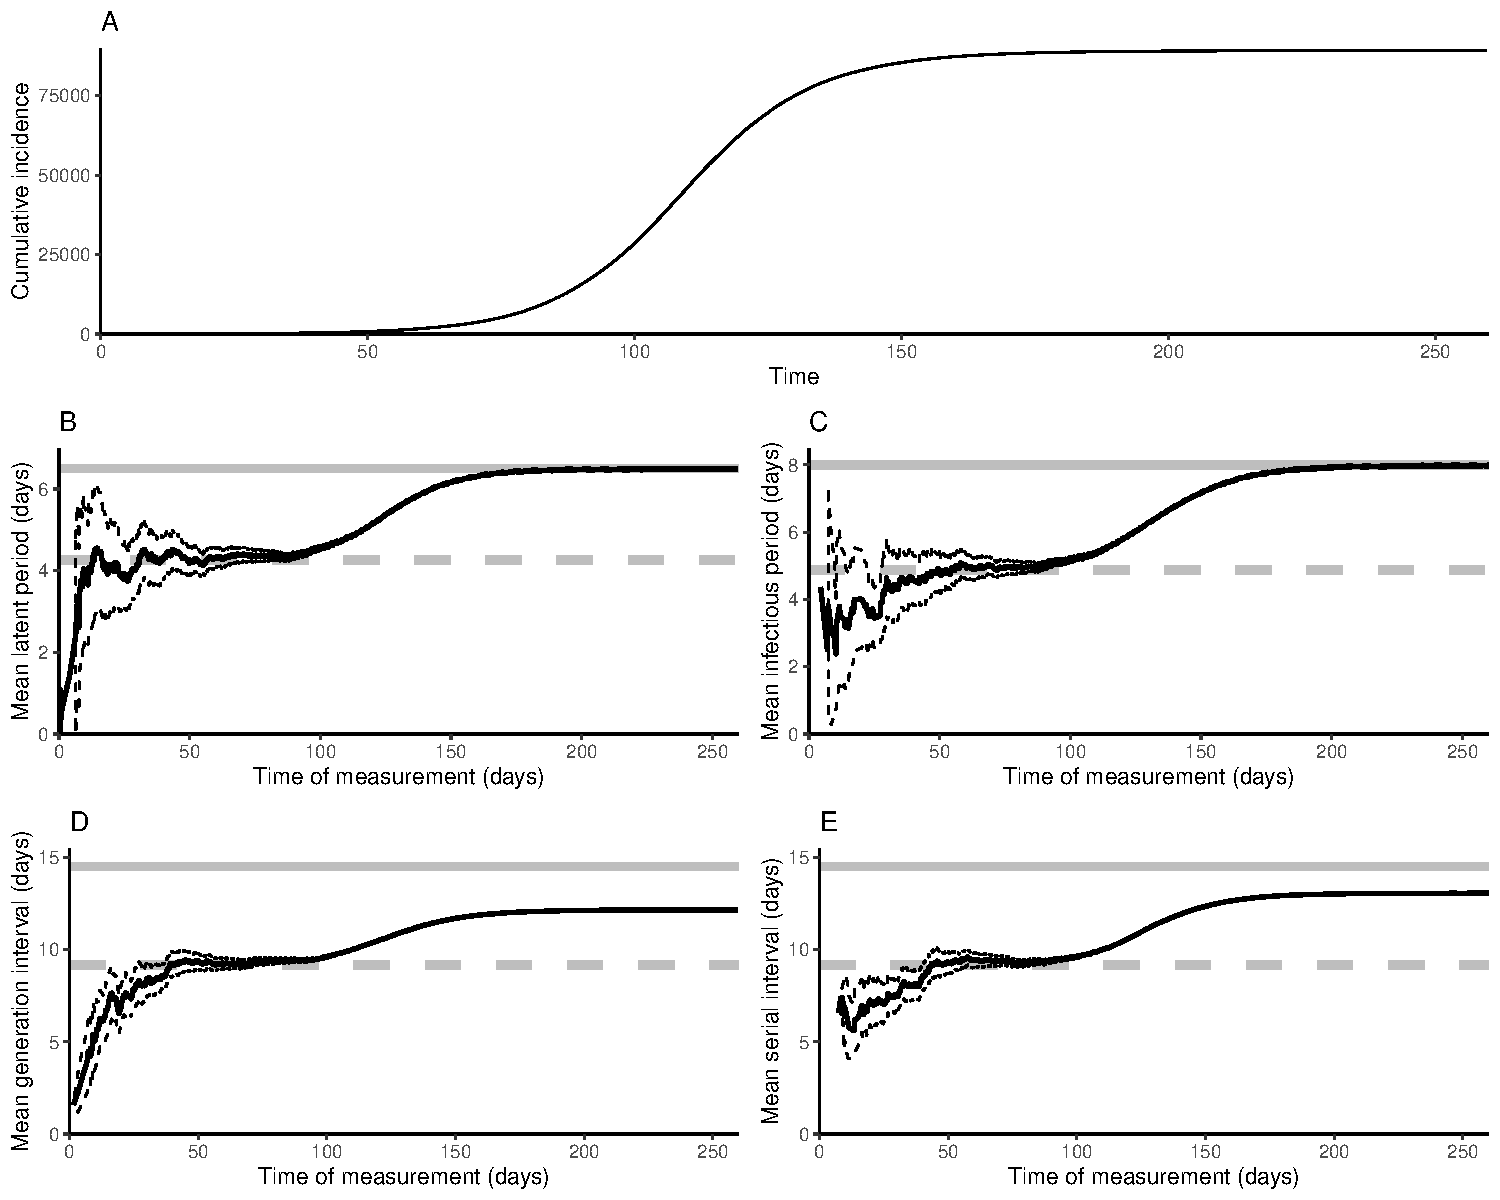
\includegraphics[width=\textwidth]{figure_seir.pdf}
\caption{
\textbf{Observed means of epidemiological delay distributions over time.}
Changes in cumlative incidence (A) and the observed mean latent period (B), infectious period (C), generation interval (D), and serial interval (E) over the course of an epidemic.
For brevity, we assume that the incubation period is equivalent to the latent period.
Black solid lines represent the observed means and associated 95\% confidence intervals, which are calculated by taking all samples until the time of measurement $t$.
Gray solid lines represent the true mean.
Gray dashed lines represent the expected mean during the exponential growth phase (see \eref{exp}).
A stochastic SEIR model was simulated using the following parameters: $\mathcal R_0 = 2.5$, $1/\sigma = 6.5\,\textrm{days}$, $1/\gamma = 8\,\textrm{days}$, $N=100000$, and $I(0)=10$.
}
\label{fig:seir}
\end{figure}

Typically, epidemiological delay distributions are estimated by using \emph{all} available measured samples.
Then, the observed delay distribution $f_{\tiny\textrm{obs}}(\tau|t)$, which takes into account all measured delays until time $t$, can be expressed as an average of the truncated cohort delay distributions $c_s(\tau|t)$, weighted by the size of cohorts $i(s)$ and the probability that both epidemiological events of interest will occur between time $s$ and $t$:
\begin{equation}
\begin{aligned}
f_{\tiny\textrm{obs}}(\tau|t) &\propto \int_{-\infty}^{t-\tau} c_s(\tau|t) i(s) F_s(t-s) ds\\
&= \int_{-\infty}^{t-\tau} i(s) f_s(\tau) ds
\end{aligned}
\end{equation}
Therefore, the observed delay distribution at time $t$ depends on changes in the size of cohorts $i(s)$ as well as changes in the forward delay distributions $f_s(\tau)$.
Changes in forward delay distributions may reflect disease dynamics (e.g., shortening of generation interval due to susceptible depletion \citep{champredon2015intrinsic}) or changes in the external factors (e.g., shortening of symptom onset to confirmation delay due to improvement in case identification).
Within-individual delay distributions that are intrinsic to the natural history of a disease (e.g., incubation period) are unlikely to vary across cohorts at the time scale of an epidemic.

Early in an epidemic, the incidence of infection, and therefore the size of cohorts, is expected to grow exponentially at rate $r > 0$: $i(s) = i_0 \exp(rs)$.
If cohort size is growing exponentially, we expect right censoring to be important: in other words, for fast-growing epidemics (high $r$), there will be a strong bias to observe shorter intervals;
this bias applies too \emph{all} epidemiological distributions.
This effect is shown in \fref{seir}.
Stochastic simulations of a Susceptible-Exposed-Infectious-Recovered (SEIR) model show that observed mean latent period, infectious period, generation interval, and serial interval increase through time.
Eventually, the observed mean latent and infectious periods (but not the serial interval or generation interval) become unbiased.

We can estimate the bias due to exponential growth.
Assuming that the realized delay distribution stays constant across cohorts during this period ($f_s(\tau) = f(\tau)$), 
the observed delay distribution during the exponential growth phase $f_{\tiny\textrm{exp}}(\tau|t)$ is equivalent to the realized distribution weighted by the inverse of the exponential growth rate \citep{britton2019estimation}:
\begin{equation}
\begin{aligned}
f_{\tiny\textrm{exp}}(\tau|t) &\propto f(\tau) \int_{-\infty}^{t-\tau} \exp(rs) ds\\
&\propto f(\tau) \exp(-r\tau) \\
\end{aligned}
\label{eq:exp}
\end{equation}
These estimates are shown by the dashed grey lines in \fref{seir}: after initial transients, the observed means converge toward the expected exponential-growth values before increasing again as the epidemic no longer grows exponentially.

The observed mean generation and serial intervals remain biased even at the end of the epidemic (\fref{seir}D--E) because the forward generation-interval distributions vary across cohorts --- generation intervals become shorter as the proportion of susceptible population decreases \citep{champredon2015intrinsic}.
The observed mean serial interval is slightly higher than the observed mean generation interval near the end of an epidemic because an infected individual with a short latent period (and shorter incubation period) is more likely infect others by transmitting faster (therefore, shorter generation interval) during the susceptible depletion phase; therefore, infectors are more likely to have shorter latent/incubation periods than their infectees.
Intervention measures are also likely to introduce bias towards shorter generation and serial intervals because they reduce the mean infectious period --- individuals that are quarantined or hospitalized can no longer transmit.

\begin{figure}[!th]
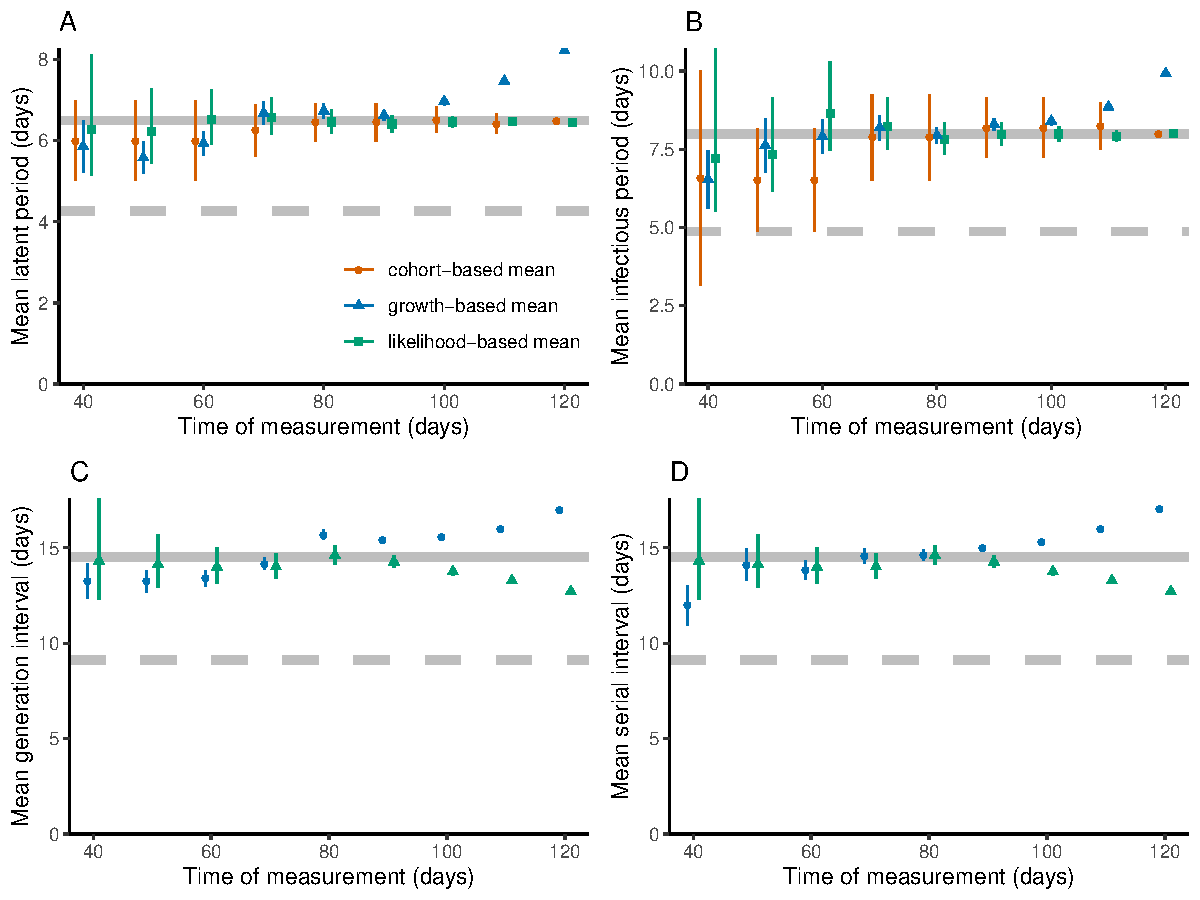
\includegraphics[width=\textwidth]{figure_seir2.pdf}
\caption{
\textbf{Estimated means of epidemiological delay distributions over time.}
Changes in the estimated mean latent period (A), infectious period (B), generation interval (C), and serial interval (D) over the course of an epidemic.
Blue solid lines represent the estimated mean and associated 95\% confidence intervals at each time of measurement using the growth-based approach.
Red solid lines represent the estimated mean and associated 95\% confidence intervals at each time of measurement using the cohort-based approach.
Gray solid lines represent the true mean.
Gray dashed lines represent the expected observed mean during the exponential growth phase calculated using \eref{exp}.
A stochastic SEIR model was simulated using the following parameters: $\mathcal R_0 = 2.5$, $1/\sigma = 6.5\,\textrm{days}$, $1/\gamma = 8\,\textrm{days}$, $N=50000$, and $I(0)=10$.
}
\label{fig:seir2}
\end{figure}

\eref{exp} suggests a seemingly straightforward way of correcting the bias -- by weighting the observed distribution by the exponential growth rate:
\begin{equation}
f(\tau) = f_{\tiny\textrm{exp}}(\tau|t) \exp(r \tau).
\end{equation}
Similar forms have been suggested by other studies \citep{britton2019estimation, park2019inferring} and have been applied in estimating epidemiological delay distributions during the COVID-19 outbreak \citep{nishiura2020serial, linton2020incubation}.
Our simulations show that the growth-based approach does not work very well for estimating the mean delay (\fref{seir2}).
Although the estimated mean delay is consistent with true mean, the estimates are unstable and the associated confidence intervals are inappropriately narrow.
Once the exponential growth phase is over, the assumptions of the growth-based approach no longer apply, and we overestimate the true value.

Alternatively, we can account for the bias by ensuring that the right-censoring does not exist in the sample:
instead of using all samples that have been collected until the time of measurement, we can limit our samples to cohorts $u < t$ such that both epidemiological events of interest have been observed for all individuals within cohorts $s < u$.
This approach provides an unbiased estimate of the mean delay throughout the epidemic and the associated confidence intervals contain the true value (\fref{seir2}).
However, this approach cannot be applied to generation or serial intervals because we do not know how many individuals each person infected exactly (and therefore we cannot evaluate whether the right-censoring exists within a cohort).

Finally, we can account for right-censoring explicitly by using a likelihood-based method based on \eref{cohort} while assuming that the forward delay distribution does not vary across cohorts.
Like cohort-based means, likelihood-based means are consistent with the true mean and the associated confindece intervals contain the true value.
Note that the confidence intervals of the likelihood-based means are narrower than those of the cohort-based means because we are able to use all available data, thus providing more precise inference.
Our likelihood-based estimates the mean generation and serial intervals eventually underestimate the true mean as they do not account for changes in forward delay distributions across cohorts.

\section{Applications: incubation period distribution of COVID-19}

Here, we revisit early-outbreak estimate of the mean incubation period estimated and assess the degree of bias in this estimate.
\cite{backer2020incubation} 

The estimate is based on travelers leaving Wuhan, China between January 2--23, during which the epidemic, and therefore the number of infected travelers, was likely to have been growing exponentially.
Their estimate of the mean \emph{observed} incubation periods of 6.4 days (95\% CI: 5.6–7.7 days) is expected to be biased due to right-censoring.
To assess the presence of bias, we apply their method to infer the probability distribution of infection time for each traveler and compare growth- and cohort-based means with the observed means over time (see Methods for details of this section).

\begin{figure}[!th]
\includegraphics[width=\textwidth]{figure_backer.pdf}
\caption{
\textbf{Potential bias in the early-outbreak estimate of the mean incubation period.}
(A) Comparisons of the observed mean incubation period using all available samples and the cohort-based mean incubation period.
Gray solid line represents the growth-based mean incubation period.
Gray dashed line represents the mean incubation period estimated by \cite{backer2020incubation}.
(B) Relative bias of the mean observed incubation period with respect to the cohort-based mean incubation period.
Gray solid line represents relative bias with respect to the growth-based mean incubation period.
Gray dashed line represents the $y=0$ line.
Relative bias is calculated as $\textrm{(observed mean incubation period)/(bias-corrected mean incubation period)} - 1$.
}
\label{fig:backer}
\end{figure}

\fref{backer}A compares the observed mean incubation period, which uses all available measurements, with the cohort-based mean incubation period.
Consistent with our simulations, the cohort-based means are generally higher and have wider confidence intervals (see January 13--24 in \fref{backer}A).
For example, on January 24, the cohort-based mean incubation period is 6.9 days (95\% CI: 6.0 -- 9.1 days), whereas the observed mean incubation period is 6.3 days (95\% CI: 5.6 days -- 7.4 days).
The cohort-based mean also matches the growth-based mean: 7.3 days (95\% CI: 6.2 -- 9.9 days; see solid gray line in \fref{backer}A).
On January 25, two estimates completely overlap because they both use all available samples; a sudden decrease in the cohort-based mean indicates the presence of right-censoring.
Since \fref{backer}A compares the marginal posterior distributions of the means, it does not allow us to assess whether the naive mean is lower than the cohort-based adjusted mean -- the overlapping confidence intervals do not necessarily imply that the differences between the observed and the cohort-based means are statistically unclear \citep{dushoff2019can}.

\fref{backer}B compares the relative bias of the observed means with respect to the cohort-based adjusted means.
We find clear and consistent bias between January 14--24;
the median estimates of the bias range from 8\% to 20\%.
These estimates are also consistent with the amount of bias that we calculate using the growth-based means: 12\% (95\% CI: 6\%--26\%).
% Overall, our results indicate that the early-outbreak estimate of the mean incubation period of COVID-19 by \cite{backer2020incubation} was likely to have been biased.
We expect a similar order-of-magnitude amount of bias to apply to estimates other epidemiological delays for COVID-19 that do not explicitly account for right-censoring.

% For example, if the observed incubation period follows a gamma distribution with mean of 6.5 days with standard deviation of 2.6 days \citep{backer2020incubation} and the epidemic grows exponentially at rate 1 per week, the true incubation period will have a mean 7.6 days.

\section{Discussion}

Understanding the time delays between epidemiological events is a key component of statistical and modeling efforts to predict and control infectious disease outbreaks.
However, estimates of epidemiological delay distributions can be systematically biased during an ongoing epidemic due to right-censoring.
Generation and serial intervals can be subject to additional biases due to susceptible depletion and therefore are more difficult to estimate.

We compare two approaches for correcting the right-censoring bias: growth-based approach and cohort-based approach.
While the growth-based approach provides a simple, intuitive way of assessing the bias present in the estimate, it is unstable as it is overly sensitive to long intervals and assumes that the exponential growth rate is exactly known.
In practice, the exact period of exponential growth is difficult to determine \citep{ma2014estimating} and therefore, the growth-based approach may perform poorly.
We recommend against using growth-based approaches.
The cohort-based approach provides unbiased estimates throughout the course of an epidemic.
In practice, using only a subset of available samples may not be ideal as it leads to less precise inference;
we recommend using likelihood-based methods that explicitly account for right-censoring analogous to \eref{cohort}.
Nonetheless, comparing the cohort-based means and the observed means still provides a viable way of estimating the strength of the bias in the inferred delay distribution as we demonstrated in our example.

Our results indicate that the mean incubation period of COVID-19 was likely to have been underestimated during the early outbreak.
However, there are other sources of biases that we did not consider:
\cite{backer2020incubation} assumed that the infection time of an individual is uniformly distributed between the first and the last exposure date.
Given that the incidence was exponentially growing in Wuhan, China during that period, the travelers would have been more likely to be infected towards the end of their exposure period.
Their uniform prior assumption is likely to have underestimated the infection time, which, in turn, would have overestimated the incubation period.
Therefore, the downward bias caused by right-censoring and the upward bias caused by the uniform prior may cancel out.
Other estimates of the mean incubation period for COVID-19 that do not account for right-censoring are also likely to be biased.

As of writing this paper (April, 2020), researchers are continuing to estimate epidemiological delay distributions for COVID-19 but the problem of ignoring right-censoring prevails.
We strongly suggest considering all sources of potential biases and recalculating these distributions.
While the amount of bias is likely to be small ($\approx$10\%--20\%), making precise inference on epidemiological parameters will allow us to assess the outlook of the pandemic more accurately.

\bibliography{censor}

\end{document}
